% Created 2023-03-07 Tue 16:09
\documentclass[9pt, b5paper]{article}
\usepackage{xeCJK}
\usepackage[T1]{fontenc}
\usepackage{bera}
\usepackage[scaled]{beraserif}
\usepackage[scaled]{berasans}
\usepackage[scaled]{beramono}
\usepackage[cache=false]{minted}
\usepackage{xltxtra}
\usepackage{graphicx}
\usepackage{xcolor}
\usepackage{multirow}
\usepackage{multicol}
\usepackage{float}
\usepackage{textcomp}
\usepackage{algorithm}
\usepackage{algorithmic}
\usepackage{latexsym}
\usepackage{natbib}
\usepackage{geometry}
\geometry{left=1.2cm,right=1.2cm,top=1.5cm,bottom=1.2cm}
\usepackage[xetex,colorlinks=true,CJKbookmarks=true,linkcolor=blue,urlcolor=blue,menucolor=blue]{hyperref}
\newminted{common-lisp}{fontsize=\footnotesize} 
\author{deepwaterooo}
\date{\today}
\title{Wired Behaviors}
\hypersetup{
  pdfkeywords={},
  pdfsubject={},
  pdfcreator={Emacs 28.2 (Org mode 8.2.7c)}}
\begin{document}

\maketitle
\tableofcontents


\section{先前的:精于试探拿捏别人,一天试探拿捏别人100 遍}
\label{sec-1}
\begin{itemize}
\item 推荐信:【帮点儿小忙,一定索要回报】她是写了,但她把别人看成个 loser, 把给别人的推荐信一定写成距离别人千里之外。如此,仍能强势索要回报,要别人开车去接她回家。后来我有四封推荐信,也把有四封推荐信的提交过了申请的网页给她看过,她的这一封也不是必须的,因为别人会有多余的。
\item 为试探擦边界,想开别人的车,把别人丢市中心走回去
\begin{itemize}
\item 然后她第一时间问【先把你放进不得不走回去的恶劣环境,再试探比较容易成功?】:想开别人的车。回来她自己也说,两三个月之内,她自己也被丢市中心过,她也是自己走回去的。【真难相信,若是她自己也真走过,短时间不到三个月之内,她不会记得?还会把别人推荐上车,让别人也再走一回?】她报复开心地说,那天我终于成了 poor baby。我严重回复了她的试探:不可能。我不可能把没有她保险的车给一个【可能没有驾照】没有任何美国驾驶经验的人开。她太作梦了,她请另谋出路【买二手车,租车,随便她】。别打我的主意。
\end{itemize}
\end{itemize}
\section{故意不理人,永远是前家门的最后一步,不得不回,最后一秒回复别人的消息,任何消息}
\label{sec-2}
\begin{itemize}
\item 可见这个人的内心得有多见不得人,多敏感才会如何极端的保护她自己【而实际上,这个人从来不清白】,却把别人恶心羞辱得要死,把别人,很多次帮助过她的人,在她那里,从来都只是她羞辱凌迟的对象,她还真高贵。。。。。太犯贱了。拿捏别人拿捏得过了分。
\item 她一次写不完作业,是【提前十分钟,在她,还算是比较好的一次了】回复别人的消息
\item 别人的关心问候在她那里也从来是她的最大耻辱,她一定在进家门前最后一步回复【不得不回的时候,回最不重要的消息】。别人,永远,关心问候的消息,都是,她的最大耻辱。
\item 故意凉人,既发消息给别人,还能故意羞辱别人一样地故意不理,不止一回,她认为别人傻,没有自尊,任由她作贱羞辱凌迟
\end{itemize}

\section{恶意抹黑、毁灭一个人的名声:2014 年秋天;和现沦陷了的可怜人室友}
\label{sec-3}
\begin{itemize}
\item 我到前天晚上才终于想明白,她这个卑微的早已经沦陷了的可怜人,每天所干的事是,想千方设百计故意叨难你,以试图以她个人的叨钻难缠行为抹黑你,一个正常普通人意外拥有的名声。
\item 亲爱的表哥,她不是个人成名后历史上,第一个如此对待你活宝妹的,2014 年秋季学期,作为一个个人,被先前的学校和系里,也如此类似不公正对待过。只是因为方式不同,现室友伪装得深,离开校园后,狠久没有这样的室友,没有经验,没能及时反应过来。
\item 但,个人生活中,她是伪装得最无古,城府最深,属马狮子座,最为强势,也最扭曲了别人的人格尊严,她的身份地位最为卑微,是个早已沦陷了的可怜人,靠身体发文章,发文章的数量(她对我自称,她国际上发表了28 篇文章)受身体检验。但她强势心狠手段毒辣。心机女的手段总是狠多,她既分身,极有可能只在家里作这样一个叨钻难缠,她既要别人生活中帮助她,她可以用车购物,她还要极不人道地故意一再作贱别人的尊严。叨钻女的本性暴露无遗。
\end{itemize}
\subsection{简短陈述 2014 年秋天的情况}
\label{sec-3-1}
\begin{itemize}
\item 对于个人的什么时候成名,如何出名:作为同任何大众一样的卑微个人,我并没有很清楚的认识,那时的自己也狠年轻不经世事,不明白为什么会出名,以及不曾期待意外到来的名,会给自己带来什么。
\item 2014 年秋天,先前的小学校UI 应该更多的是认为:一个国际留学生,却出奇【我自己也不知道是为什么?】地有比较大的名声,系里是有位某个专业方向上的大牛的,或许系里是认为作学教育系统的某个专业方向的牵头人,系里或觉得,若能及早灭掉一个普通国际留学生由于任何原因,所拥有的名气,或许是当时他们所认为的更为正确的做法?
\item 于是2014 年秋天,作为一个最为普通,甚至是发展还点儿迟缓滞后的国际留学生,仍存在文化差异,认知问题等,便狠狠体验了一回,在出国留学的异国他乡,被系里专业课上一个小集体,搞孤立和差异对待的不幸记忆。
\end{itemize}
\subsubsection{系里专业上导师对自己抹黑灭名的方式是 \textbf{【项目专业能力上的指鹿为马,强加抹黑】} :}
\label{sec-3-1-1}
\begin{itemize}
\item 秋天某次 LED Tower Light show (是秋天的9 月或是 10 月), 是在校园中心用学生宿舍楼和窗子,每个里放LED 灯大型演示。那天下午,导师一定要求使用我有 Linux 系统的电脑来演示,这个项目里的任何同学都没有我所使用的那个 Linux-mint 系统版本?于是导师借一定要用我的笔记本电脑,将我捆绑在那天晚上的演示现场。但演示 demonstrate 的过程中,导师故意中途演示表演失败,这样,导师或系里便成功让,整座校园的师生认为【甚至有着求扩散传播的动机目的?】:这个国际留学生,专业能力不足,她项目【实则只是人被导师变向绑在现场】大型演示中途熄火,这让我作为一个国际留学生的专业能力,在整座校园【甚至接下来的整个求职生涯,可能延伸扩及的面,已经被所受教育的这个校园,掐死了一半】被强加一个巨大的问号。但实际上那个演示展示项目,是导师其它学生的项目,从来不是属于我的项目,与我没有半点儿关系。演示失败是导师故意的。除了导师一定要用我的电脑把我捆绑到演示现场,将这个演示中途失败的结果表象,强加强按在这个国际留学生的头上,那个项目与我半点儿关系也没有。但作为一个国际留学生的专业能力,却在整座校园,被人为强加一个?问号。自己后来的找工作等,也因为学校的恶意阻拦,招告天下的态度而遭受诸多挫折。 \textbf{国际留学生,来到这里读书,说到底,就是希望毕业了能够至少是顺利地找到份工作,好好生活发展,谁曾想望,在一所鸟不拉X 的小地方,读个书,拿个学位,临毕业了,还要被学校系里,把个人的发展给堵死、整死一半?任何人任何国际留学生都不会希望这种情况发生在他自己身上,但事实是,它就是可能会发生在任何国际留学生个人身上。}
\end{itemize}
\subsubsection{人际沟通合作能力上的打压:}
\label{sec-3-1-2}
\begin{itemize}
\item 那个秋天 \textbf{系里课程《Senior Design》上:呈现出两种可能的结果打法} :一个小组的项目, 大概有四到五个成员。
\item \textbf{一种打法是:如果分配给我的组里的项目任务,我没能做出来,那么就打成是专业问题,专业成长能力不足【潜台词:不适给予提供工作机会;求扩散,打压这个人的发展】} ;
\item \textbf{另一种打法:如果我做出来了} ,那就是由代课老师指挥,由那个本科生女组长负责协调,将这个合作项目通过组长协调组员的一再擦边界,把别人的合作项目, \textbf{通过小组长一再与组员的协调与擦边界,打歪打成了人际沟通问题,这个人这个学生,沟通能力不足,不能够与他人合作【潜台词:不能与人很好沟通的人,发展应该受到限制】} 。
\item 总结就是, \textbf{无论你在这个项目里的专业能力,人际沟通能力如何表现,他们都一定鸡蛋里挑骨头的做法,就是一定要纠出你的错来【不允许你发展,逼你读博士】} 。最后是因为自己的项目安时完成得很好,这个与本科生一起做的小组项目就,被打成了人际上的不能与人沟通,被代课老师要求,从合作项目里独立出去,我的项目被代课老师要求自己独立完成【另一个原因是, \textbf{项目也包括很多文书读写要求。国际学习受制于语言,语言文献上的读写能力,相比于计算机程序员的编程能力,可能会是他们更大的挑战,他们想要挑战你,以期待纠出你更多的不足} 】。
\item *项目过程中,被项目小组搞围攻粗暴对待*: 
\begin{itemize}
\item \textbf{无限放大一个小组成员缺点的做法是:被代课老师指导,小组长负责协调带动其它组员的,就是组里的每个成员都假装装作拥有你身上的一到二个缺点,当他们故意通过邮件或是某种方式将你身上也存在的这些缺点集中一一申明表明表现出来,故意制造焦点,故意制造社会关注点,那么所有其它组员共同执行代课老师的要求一起合作,就把你国际留学生一个个人身上十个八个缺点都一一放大出来,求焦点求关注,求社会工业界合力共同阻碍这个人的发展,逼国际留学生读博等,} 为的当然是阻止这个人的发展。
\end{itemize}
\end{itemize}
\subsubsection{系里对他们如些粗暴对待国际留学生,有自知之明吗?有,但打擦边球,为他们自己准备好借口}
\label{sec-3-1-3}
\begin{itemize}
\item 导师的借口是:我就是只是用了你的电脑,演示现场还有其它全部都是美国学生,因为项目里就是美国学生,只有你一个国际学生,难道我需要从哪里去拉个国际学生来给你作伴吗?
\item Senior Design: 课的借口是:代课老师只有硕士学历,是院系里学历最低资历最低,专门负责系内各类脏活有损大牛们名誉的打扫卫生的活儿的,12 年秋天上他的C++编程课,也被这个代课老师当着全班同学的面,因为一个 segment-fault 的程序崩溃上课前问老师,被当场狠狠羞辱过,当时课堂上趴桌子上哭了一堂课 \textbf{【规模小的学校,野鸡学校,这种情况时常会有发生】但好些的学校,不像小规模学校没有完整的或是根本没有一个相对成形的管理体系,又或是受控于一个独裁者,被弄小灶般的恶意来顿也就狠够你受一阵子的} 。硕士教教本科生,资历相对欠缺,系里的态度就是:发生这种情况,谁也不愿意,但无可避免。他们只可以总结教训,不负责任何其它。 \textbf{国际留学生,面对别人故意打压限制你的手段,面对别人只总结教训不负责已经发生过的事的结果,你能强求说:我在这所学校这个系,遭受了这些不公平,你必段得给我补偿培偿一份工作吗?作梦吧,永远不可能。就是,发生在任何一个个人身上,就是任何个人个体的极大悲哀。这样的结果,是任何国际留学生不想,也不愿意看见的} 另一个他们的护身法是:把责任推泄给组员。他们是一群本科生不懂事的孩子,代课老师也不知道他们出于任何原因,合作团体对一个国际留学生构思执行实施了围攻粗暴对待。
\item 没有读博:厌倦了那个环境,想逃跑。
\end{itemize}
\subsubsection{再补充一点儿:2014-2015 年学年居住环境:留学美国好多年,女房东的学历社会地位最高,提供的自己寻找到的居然环境却是最差}
\label{sec-3-1-4}
\begin{itemize}
\item 14 年7 月找租住地方的时候,原本还有个女孩可以合租一个 apartment, 但事后知道被她室友的导师稍微影响了一下,她室友是不能搬走还是怎样,不能再出租,就只能 \textbf{租到学校某个女老师大街上的一个 house 里一个最小的房间,房租比较贵,2014 年8 月,\$300 一个月【她收的房租奇高,后来知道他们的目的就是想把原本手头不宽余的临毕业留学生弄 broke】} ,但因为当时不再有其它出租 available,最小的房间,四面一面长面有个小窗户,其它三面一个短面是另一个室友房间,另两两,一个长面摆的自己单人床,但墙的另一侧又大家三个女生合用的一个公用洗手间的 show-head. 另一个短面的另一侧是洗衣房,有洗衣机烘干机和水槽。
\item 地址是: \textbf{115 N Jackson st. ID USA}
\item 这个老师还给她自己留了一个房间,偶尔月头来收房租的时候会住一晚,同样负责调整?打听她的租客的一些信息?或她想要如休左右一下她的房客该如何行事,调风向?
\item \textbf{共同一面墙的室友是如现室友般是夜行动物,晚上厨房做一晚饭,早上水槽全占满小厨具;她也专门晚上洗衣服烘衣服。她是专门负责晚上故意吵别人休息的。} 某次女老师来还暗示我可以帮助她洗水槽厨具?我不明所以,我自己做饭从来一个菜一个锅一口饭碗最简单几个,几分钟做完,十几分钟吃完清理完,为什么我需要帮她洗呢?我没有。
\item 早上的情况是, \textbf{前门街边一个房间的女生,每天早上 6:00am 起床洗澡,头发长,女大学生爱干净,洗的时间长。她每次洗澡需要洗二十多分钟半个小时左右} 。
\item 这样, \textbf{每天早上6:00-6:30 被这个女生吵醒;几乎每天晚上,再被这个共一堵墙的室友洗衣服烘衣服,或是厨房做饭做吃的吵半夜} 。
\item 我无意去说, \textbf{当时的那个房东UI 学校的女老师是代表哪方立场,她是UI 的某个专业的代课女老师,但或许她所代表的并非UI 立场} ,我无法定论。因为不同于专业上,同一个院系里的老师师生真正管理层管理者是谁等,大家打听得比较清楚一点儿。真正当权的或是和事佬,真正干政作决定的,实则躲藏在背后隐藏保护得比较深的人。
\item \textbf{很想去相信这样的居住环境,几个租客是巧合是偶然,但那是永远不可能的} 。但是 \textbf{不明白为什么从网络上6 7 月7 月找租住地的时候,就会被限制到这一个女老师的名下。}
\item 这个女老师没能协调好她的租客,或是她的故意。 \textbf{国际留学生,要怎么样才能够擦亮双眼,即便是大学里的教授,也是会各种作恶,来环境威逼压迫一个国际留学生的学习与生存的?}
\item 14 年的秋天还是相对好点儿。14 年底的一场变故, \textbf{15 年春天居住地重要邮件,感觉是在,都在丢失} 。寄邮件的地方说,他们什么时候寄出来的。但是早该到达的邮件呈现出丢失状态。这里最主要是强调: \textbf{当一个人处于低谷,正在异国他乡遭受一些感受着被周遭环境不公平对待的变故,相关的重要邮件一再丢失,都会成为一种环境的威协与威逼力量,协迫办量,压迫和威逼异国他乡远离亲人的留学生的内心与精神} 。从2014 年12 月底到15 年3 月一份不被公平对待的遭遇相对结束,两三个月,三个月不到的时间, \textbf{对异国文化(不是自己出生生长熟悉的环境与处事方式,不明白)没有足够的认知,不知道事情接下来会如何发展,不知道被不公正对待的迫害,是否因为一再丢失的邮件,会把自己一再推入险境。}. 不知道接下来会怎么样,感极端忧虑,那两三个月的状态都不是很好。却同样不知道该如何才能得到别人的帮助。想来想去,或许无意中由于任何原因得的那点儿名能够稍微帮点儿忙。另则, \textbf{这是一所鸟不下蛋的荒芜之地,地方小,感觉世面似乎也小,各类幺蛾子极多} 。或许上到网络上求助,能够得到一点儿关注,或是好心人的帮忙。于是上网创建贴号发贴:但想要得到的回复都没有。
\item 那个春天的两三个月狠漫长。我想, \textbf{如果一个学校能够有真正可以帮助国际留学生,教导或是提供必要的建议,该如何处理这类极端事件,会好受很多。}
\item 可是 \textbf{那个时候的环境是孤立的。在漫长的等待中,煎熬中等待了直接一件事情的结束。接下来,便是逃跑,毕业了便永远离开,想要永远远离那个地方。在那个地方再多呆一个学期,都是困难的,完全不可能留下来继续读博士} 。
\item \textbf{这一年的居住环境,是室友早晚的作息环境接下来十年里都几乎是最差的} 。除了现室友是隐藏最深,属马狮子座,三十三四岁,感觉极端强势,不为他人考虑,人品狠差。她自己可能遭受过网络暴力或是舆论暴力,或是极深的情感伤害,她或没能真正从那种伤害中走出,或是畸形心理,使得她一再将这种极端暴力做法态度一再强加给她身边的人。不过,现室友的事是发生在自己又成长了好多年,相比于当年心智成熟强大了狠多。很多事情可以试着努力去理解,但没有任何愿意自已的好心被别人一再拿捏,或是利用。
\end{itemize}

\subsection{再来看现室友:如2014 年秋天个人的遭遇是学校立场般,她,所代表的是WSU 的学校立场吗?不,她极端辱没了WSU 的校园文化。WSU 拥有上百年(125 年)的教育历史,公平透明,拥有极好的国际留学生学习环境}
\label{sec-3-2}
\subsubsection{作案手段手法:与2014 年秋天的遭遇院系集体,个人遭遇,如出一辄:有过之而不无及,隐藏深,手段狠,制造舆论焦点,恶意抹黑他人声誉}
\label{sec-3-2-1}
\begin{itemize}
\item 她是那个拿她自己土耳其国家的工资,也就是拿不到WSU 任何工资,出来合作一年,以免费劳动力服务于WSU 的某个项目。 \textbf{隐藏于她国际合作人公益人(因为她没有资格,拿WSU 的任何工资)身份,【想起来该是多么大公无私,勇于献身的精神】不容易被他人发现或是怀疑:}
\item \textbf{只施加对一个人的恶意与暴力【只限于在家里,只对一个人,只对这个人施恶】} 。她在家里几种模式,可以想见,她在工作的地方,表现相对得体。在她工作项目上,她最卑微,比不上博士后拿美国导师的工资,比不上博士,有大好将来。 \textbf{她应该是不至于白天在实验室大象撞山把水龙头任何时候,哪怕半夜也开到最大,撞山响的}
\item \textbf{用实验室公益人身份,和工作社交场合,所展现出来的正常,来维护她【成熟正常人形象】} :足够成熟,社交礼仪得体。 \textbf{任何时候,似乎都不至于。对其它任何人,怎么样}.
\item \textbf{但实则在家里,在只有一个室友的地方:她分身} ,她如2014 年秋天项目里的同学般,无中生有【你没有错,故意制造强加给你各种错,甚至一度恶杀一个人正常的心智反应】;恶意寻三找四,故意制造各种事端, \textbf{不惜牺牲她个人在家里的形象,为的只是,抹黑你,一仍残存着一些在外名声的人。就是,以她一已之恶,之黑,来故意恶意抹黑别人} 但是因为她国际公益人身份,没有资格,拿不到WSU 一分钱工次,充当免费劳动力在这里一年,她在工作和社交场合的,【可以合理理解与想像】,正常的,得体的,绝不至于大象撞山的得体方式,保护维护他的正常人身份形象。
\item 但她保护自己的方式是: \textbf{消息里对你各种冷落,把你当作是那个坏事做尽,不值得她这个室友回复消息或是尊重的天下最坏室友,各种冷漠,以予理采,甚至施加暴力【5-7 天故意躲她房间】} 。她把这种手段,当作是她的自卫,与对外宣称的他的立场:恶室友,不足以为伍,感觉羞耻。
\item \textbf{故意制造焦点、炒作舆论:【5-7 天故意躲她房间】} 她,初到美国不足三个月,以一个国际异乡人的身份,发给了一场舆论风暴,想要恶意抹黑一个人的声名。实则,她才是那个有着诸多问题的可怜人。
\end{itemize}
\subsubsection{她,在个人住宿场所的个人行为,极端辱没WSU 校园文化。她是个案,是特例,无力无法,也不应该代表 WSU 校园官方立场}
\label{sec-3-2-2}
\begin{itemize}
\item 那么现室友,对一个同为国际人的室友,如此恶意行为,她代表的是哪方观点,或是意见?她能够代表传达的是WSU 对待一个稍微还残存点儿名声的先前国际留学生的立场吗?不,她的做法,极端辱灭了WSU 的校园文化。
\item 她只是一个拿她自己土耳其国家的工资,出来做义工,积攒经验的,某个导师名下一个做义工,求机会学习这里先进项目经验的合作人。她甚至不是这里WSU 的博士后,因为她的工资由她自己找,是她自己的国家支付她,或者也可以简单地理解为,她自费,出来一年,在学习这里的先进经验的。
\item 如果说,2014 年秋天,更多代表的是以前先前的小学校,作为拥有一个专业方向上一个大牛的系,一个教育机构,对一个微小个人的围攻,不人道行为。【这里我也申明一下自己作为个人的感受】
\begin{itemize}
\item 【这里我也申明一下自己作为个人的感受】:我个人认为, \textbf{任何时候,一个系,一个群体,一座校园,对任何一个个人,哪怕是这个个人因为某种连她自己也不明白的原因意外拥有某种名声,对这个个人,施行不公正的群体围攻,都是不公正、不人道的行为。会给有着(哪怕是足够成熟,没有)文化差异的国际留学生的生活造成太大的困扰与不公,会影响其人对这个系,这个校园,或是这个国度的文化认知,或产生偏移错位} 。
\item 很多有点儿了解或是社会经验的国际留学生申请者, \textbf{哪怕是需要支付的学费相对稍微贵那么一点儿两点儿,也都会选择校园规模相对更大,更为公平公正、透明的学校院系,是有着足够道理的} 。
\item 好的学校,公平公正管理透明的学校,哪怕是自费必须交的学费稍微贵一点儿,但 \textbf{能够真正进入到一个好的体系体制受教育的学校,是一种半步一步已经迈进顺利成功【比如,最低生存标准:至少是毕业了能够在这边找份工作养家糊口吧?】的保障。} 而以个人亲身经历,比如个人临毕业前不幸经历“野鸡”大学的某种干扰,即便是毕业了拿到了学位,工作却受到教育系统的一定程度上的牵制,接下来的生存发展就必将受到更多的限制。 \textbf{说得再精准点儿,大家喜欢讲,赢在起跑线上,选择了规模小的“野鸡”大学,原本就是输在了起跑线上;而哪怕是刚出国时必须自费,选择了一所规模更大,更公平透明,拥有良好声誉的大学,哪怕是自费,能够想得开,其实已经是,就是赢在了起跑线上,哪怕刚出国时是自费出来,但这个管理完善、成熟的教育机制,已经能够保证保障其学生,毕业了找工作、工作发展能发展得好,就是胜利!这个时候,再来回看,刚出国时的那点儿学习费用,当然会珍惜和明白,有所投资有所回报。}
\item 因为普通国际留学生,亲爱的表哥,如你的活宝妹,从小长到大,品学兼优,考研究生考TOEFL, 考GRE 申请到奖学金出国留学,生活从来都顺利平静得不起任何波澜,作梦也不会想到,在一个异国他乡,任何可能会遭受到被孤立或是恶意对待的风险可能,但 \textbf{现实往往是,在一个竞争更为激烈的发达国家,这样的事情就是都有可能会发生、降落在任何普通大众国际留学生的身上,如你活宝妹的身上。而任何降临在一个卑微个人身上的这种被区别对待,都是一次头破血流、血淋淋的教训,又或者是生活的道路与选择,在这种无形中被扭曲扭转。}
\item 出国前,常年生活在菁菁校园的人,社会阅历一般极少。所受的教育,会让大家本能地相信:天是蓝的,水是清的,这个世界总是公平竞争的。。。。。顺利地拿到去往美国发达国家的鉴证,将来的路都必将是顺利的。。。。。但实际上,不夸张的说,确实有很多在国内表现优异的国际留学生初到异国他乡,并不真的知道或是明确接下来的生活目标是怎样的,甚至该如何在另一种文化中顺利顺滑圆润地生存。如果说在国内时努力学习的目标是为了出国,那真正出来后, \textbf{并不是每个人任何时候都能够明确坚定自己的学习目标,走错走偏时有发生} 。国内所受的教育受教育过程中极少可能出现被异端对待的情况,尤其对于从来都学习成绩好,三好学习,老师同学都喜欢的天之骄子来说。但 \textbf{出来后在一个竞争激烈的发达国家,会发现连校园、教育机构与体系都并不总是公平的,“野鸡”大学,或是规模较小的学校,不公正不透明,各种作法小家子气的所谓大学,如幺蛾子般的做法都极多,对国际留学生实行、执行必要的不公正对待、歧视甚至于恶意打压等现象,狠多,并非总如国内不了解情况下发想像理想的那样:天蓝水清,总能遇见最为美好的爱情,一切都是极好极好的。。。。。就连教育体系,也是存在诸多受教育不公正的} 。。。。。【过来人经历,个人现身说法】
\item 【 \textbf{很多时候,并不是任何一个真正遭遇这种对待的人,都有足够成熟的心智与坚强意志,面对这一切} 。哪些时时报道,想不开跳楼跳桥的,是为什么?】并不是任何一个顺风顺水成长成熟的人,都想当然地拥有面对突然变故,或处理生活中的意外的能力。
\item \textbf{大体上,就把出国留学生综合素质,分为两类,一类是各种综合素质好,就算人生第一次经受一场重大打击,都可以独立顺利处理过关} ;而 \textbf{有那另一类人,必得经历过他自己人生的第一次打击,方能成长心智真正成熟起来。这后一类人,若是所经受的第一场重大打击,是在远离亲人朋友的异国他乡,缺少这些至亲至爱的人的理解与支持,必将会是一场极大的考验} 。就算能够处理过关与不能过关各占50\%, 面对那50\% 失败的结果,这边博士、博士后跳楼跳桥的都很多,有学业中途废掉,比如被导师停助教助研经费,没有了奖学金学习生活成问题,回想起回国一跟学业上学习成绩独好【所谓聪明反被聪明误:除了成绩好,其它心智成问题。或是学习好便一直读,个人爱情婚姻生活成问题恋爱结婚严重滞后等】,无法接受现状结果,想不开轻生的。。。。。实在不要太多。 \textbf{没有发生在某个人体自己身上,自已就是开心顺利的一切;真正发生在某个个人个体身上,就成为一个个体个人的极大不幸与悲哀。}
\item 亲爱的表哥,活宝妹当年不是,多么明白的应该是继续读博,为什么逃离了那个地方?那些年的自己很年轻脆弱,长年生活在象牙塔校园里的活宝妹无力消化14 处秋天和接下来15 年春天所发生的一切。当时只有一个愿望,就是永远远离那个地方。但多年以后回望,当年的自己为什么没能读博呢?只是,再多十年的成长,让自己终于能够相对公平公正不带个人情感地去回忆当年已经发生过的事,对于当年自己遭受到的那些,近十年过去,现在的活宝妹终于可以原谅和释怀,可以平静地回忆。
\end{itemize}
\item 她极端辱没了WSU 的校园文化。她所做的一切,更多的只是她个人一个卑微个人受困于成长或是心智素质,她自己个人心智性格或更多人品上的问题。她是她,她是存在于WSU 系统里的几乎最差存在。
\item \textbf{她极端辱没了WSU 的校园文化} 。相反, \textbf{WSU拥有上百年(125 年)的教育历史,公平公正透明,拥有极好的国际留学生学习环境,支撑体系,不管是学业专业上校园教学楼,随处可见二维码扫描寻找同一专业上共同写作业的小伙伴们,还是生活问题上的支撑体系【对那些真正经历人生低谷的人来说,远离亲朋好友,真正困难的时候,当然是很强的支撑体系保障学生的心理精神需求】,校园文化以及管理体系,公平公正透明,以极佳的国际留学生培养成长体系环境闻名海内外。}
\item WSU 拥有开放的校园文化。亲爱的表哥,活宝妹觉得自己狠卑微,是微不足道的尘埃。但作为最普通的平民老百姓,活宝妹仍能开怀开放地表达自已的观点认知与看法,去表达自己某方面的不公正被对待,而这里的 \textbf{公平公正开放的校园文化更为多元包容,永远都绝不至于会存在任何,对一个任何个人搞围攻施加暴力粗暴对待的可能,而更多的时候,是文化上的包容} 。是一座拥有极佳人文环境、人文关怀的国际留学生培养成长成才培育系统。从这座校园里走出去的学生,毕业生,综合素质都很好,找工作以及后来在社会上的发展也都很容易顺利成功。这样的校园文化,任何时候,绝不至于恶意对待一个国际留学生个人。国际留学生的申请者,申请的学校的基点基石,不正是严格需要这种保障保证吗?
\item 亲爱的表哥,活宝妹有时候会怀疑自己:亲爱的表哥的,你的活宝妹真很奇葩吗?为什么你的活宝妹容易遇见如现室友这样的奇葩室友?心伤!!她,只是存在于WSU 的一个最小的意外。她这样的存在,应该只能反面刷新,这座有着开放人文文化人文校园,对她,是多么地包容善待。
\item 亲爱的表哥,活宝妹有狠多话想要对亲爱的表哥表达。我先看看项目,下午或是傍晚,接下来再写完。
\end{itemize}
\subsubsection{她个人,与室友间所表现展现,她制造焦点,炒作了一场舆论背后成因分析}
\label{sec-3-2-3}
\begin{enumerate}
\item 日常生活中表现出来的品性:随时随地撒谎
\label{sec-3-2-3-1}
\begin{minted}[fontsize=\scriptsize,linenos=false]{text}
亲爱的表哥
她头脑狠灵,随时变换她表达的说话
也就成为了随时审时度势随机应变
另一种恶的情况就是,随时说谎,以最大限度地支撑她的立场

相信今天傍晚 aparment 的管理者
也亲自检测测试【比如外面站了五分钟,清楚地知道她在家抽烟了】她的撒谎应变情况
但是当管理者当她面问起,她就是立即当面撒谎否绝应变了
我相信这位管理者是,看破不说破,看她还要如此作恶下去吗?
观察过检测过,实在考查这个人的人品,相当于不说明不明说地警告过她了
她以后应该皮长紧点儿了

前天半夜两三点钟的最在水龙头
是昨天晚上十点我问起她
她先说先承认她是开到了最大(听她说想喝凉水的意思应该是喝的凉水cold 最大量,两大玻璃杯)
然后我提示说,以后晚上别人休息的时间她或许可以开小一点儿
但她随机应变,听我这建议后,她立即改口说她开得不是最大,她就是开的中小量什么的,假装是什么样的
那我见她又改口,当时就建议说,既然也不是每晚都夜间作息
或许夜间她作息别人休息之间,她可以用个容器把水先准备好。提前把水准备好
她再找借口说,她想喝凉水。。。但她自己也看了冰霜,我就没说话,她可以放冰霜里呀
然后今天再次说起,她又改口说,她想喝的是 fresh cold water from sink......
但她会小心一点儿
说到夜间两三点钟水龙头最大,她今天再绞辩一次说,她不是以为我两三点钟睡梦中醒来
她以为我两三点钟还不曾休息?!我从来至少11 点躺床上,即便偶尔因为她或没及时睡着或半夜醒来
别人是想醒着的状态;另则,她也该注意给邻居的不良影响
她就故意找借口说凌晨四五点邻居如何拍门
我说我从来没有听见过邻居恶意拍门
我说了:我们不能强求邻居怎么样,但是我们应该尽量去做好邻居 
她无语了

今天说到厨房水龙头开时,洗手间听起来会狠吵时
她也承认,她说她也早意识到傍晚我厨房洗餐具她在洗手间狠吵

活宝妹听到这话心里狠凉 
那么,活宝妹这里就有个问号:真巧,知道活宝妹跟她后面上厕所
她就刚好要喝水,还打了两大玻璃杯
她是真想喝水,还是她明知道别人半夜在用洗手间,真心更想故意吵别人?
她承认过的开的水量是cold 最大量,
那么她真正开过的是冷水的最大量,还是冷热水混合的最大量以便更吵最吵人?

今天是她在厨房放水我在洗手间测了一下
等改天她不在家,我会把冷水最大量,与冷热水混合的最大量再独自测试一遍
把她这条可能会以此夜间故意吵人的手段堵死
她以为若再这样,我自己在洗手间,可以随时测,随时录屏
\end{minted}
\item 对她人的,情感婚姻信息,无力接收消化
\label{sec-3-2-3-2}
\begin{minted}[fontsize=\scriptsize,linenos=false]{text}
亲爱的表哥
你的活宝妹观察注意到一个非常有趣的现象:

就是无论你活宝妹在室友面前
提过多少次,活宝妹是一定要嫁给亲爱的表哥的
活宝妹任何时候都是一定会嫁给亲爱的表哥的
活宝妹若是还没能嫁给亲爱的表哥
活宝妹就永远守候在亲爱的表哥的身边
在WSU 这座校园,这个小城生根发芽开花结果。。。。。

但是,哪怕是昨天我又再一次地她面前提起,
哪怕是明天,亲爱的表哥说,我们结婚吧
活宝妹都一定会开开心心地说,好,活宝妹这辈子的愿望终于达成!!!

但是,不知道现室友为什么34  岁还没有结婚
她说她希望明年她回去可以结婚,但她对活宝妹与亲爱的表哥的婚事反应
感觉她可能说的是假的,
因为无论别人千百次地在她面前提起说到,别人会希望能够尽快成婚

她的头脑,脑袋不知道哪根经搭错【还是她某方面生活经历的固执与执念】,
使得她,似乎永远接受不了,或是【别人重复了无数次的这个愿望信息】
似乎,永远无入真正进入她的意识内心
任何第一次初次了解到的人,都会印象深刻,知道这个室友是有男朋友
想要尽快结婚的状态
但是她关于别人的话与观点,反应出来的
就是别人的这条信息从来不曾真正进入她的意识
从来不曾被她的头脑真正主观接纳过接收到这条信息
是不是狠好玩儿?心理上,这是什么原因呢?

比如,在活宝妹千百次地提到会想要尽快成婚之后,
昨天再一次地说,秋天我可以申请WSU 的住宿后
活宝妹的内心突然想笑:为什么这一方面,她永远如此固执地把别人数百次传达的信息无法纳入她的印象?
活宝妹笑说:
如果活宝妹能够与亲爱的表哥及时成婚
自然是秋季不再需要申请WSU 的住宿的,活宝妹会同亲爱的表哥共同想办法解决住处问题;
如果活宝妹还没能与亲爱的表哥的及时成婚
活宝妹可能应该会去考虑:5 年读博,是否买一个相对便宜的 mobile home 之类的住处
在这座小镇扎根安家

活宝妹惊奇地观察到
原来从它人对一条信息,一类信息的反应
可以看出这个人对爱情,对情感,对婚姻的感受或是现状

不知道她,这个室友,
为什么就对别人有情感深厚的男友
别人会想要尽快成婚的信息,
永远无入真正纳入她的认知与意念
相对的,去感觉,她可能告诉我的,她的情感现状,与想明年回去后与她现男朋友结婚
也就未必是真实的
因为她反应出来的,对别人情感、婚姻的信息接纳状态呈现一个问号或是惊叹号?!!!
她为什么就固执地,永远接收不到别人有男朋友,会想要尽快成婚的这条这类信息?
你的活宝妹感觉这个方面,她的状态呈现得狠好玩儿。。。。。

爱表哥,爱生活!!!
活宝妹就是一定要嫁给亲爱的表哥
爱表哥,爱生活!!!
\end{minted}
\item 对某个方面的消息,极端过敏敏感,反应过敏,反应极端,缺乏对他人最基本的社会尊重,恶意炒作舆论
\label{sec-3-2-3-3}
\begin{minted}[fontsize=\scriptsize,linenos=false]{text}
亲爱的表哥
你的活宝妹在与他人相处的过程中
也终于可以慢知慢觉地用自己的双眼,来观察和感觉
某些方面的异常:

比如昨天晚上感觉最明显的,
哪怕活宝妹在她面前提一万次,前半个小时还在说,活宝妹有男朋友,想要尽早嫁给亲爱的表哥
这条信息,关于活宝妹情感现状的这类信息

永远不被这个怪异的室友接收,她的头脑对于这类信息,
似乎在她,像是一阵儿风,左耳进右耳出,过后了无痕迹
她的头脑,从来不曾主观想起或是意识到,
这个室友曾无数次提过
有男朋友,会想要尽快结婚
她的头脑,反应出来任何时候,
她提到过的观点,意见建议,方方面面,
她把别人当成没有男朋友的单身孤立状态 

所以,活宝妹对于她这方面,情感方面的大脑信息处理能力持一个有趣儿的惊叹号怀疑态度
读得心理学方面的书极少,不知道这方面的专家如何分析解读这类现象

同样,相对的,如她前段时间所发起的一场风暴舆论般:
为什么她可以无数次撒谎敷衍你活宝妹
极没人品不地道地:既想用别人的车,还故意各种凉别人【把别人编造成离了她不成活一样】,与别人保持距离,似乎她与别人无任何联系,同了别人的车购物却以别人为极端无耻状态
她地道一点儿,实在一起,她心有嫌弃,她不可不必乘坐别人的车去买她要抽的烟,她自已乘座公交车去不就行了,何必故意伤害别人?
她既要用别人的车,她的故意凉别人,就是一种不地道
她接下来家里故意躲房间5-7 天与室友不见面不说话,如空气般不存在不用感知

那么,为什么这类信息方面,她初到美国三个月不到的国际人
又会如何地敏感过敏,作出种种过激极端反应?
可以远远走在舆论的最前面,甚至她自己以她极不地道的国际文化异乡人身份一手发起一场舆论?

说到底,说得重点儿,她自己要么就是早已沦陷了的可怜人【她对某类信息消息,有她根深蒂固的执念,某方面的脆弱,即是她沦陷了的原因,也是她今天对这类信息极端过敏的因果结果】
要么她的情感怪异,经历非同一般【可能想到的,比如说,是否,可能,她曾早在她自己的国家经受过人肉舆论暴力伤害,或是受到过极深的情感伤害?】所以呈现出某种过敏状态?
因为她是初到美国文化异乡人身份
其实大家也就当是看了个笑话,笑笑而已。没人真把她成某回事儿

只是,活宝妹总结,原来,人的头脑,处世,对不同类型信息的不同处理方式
能够反应呈现出一个人的头脑精神与认知现状
如果不用总结多的,她,可能就是一个有故事的人吧
每个人都很忙,谁真的去在意,她的故事又到是怎么的呢?
更多的是,呈现出,对一个有故意,或受到过伤害的,可怜的人,一种本能的人性上的善,尽量体谅与包容

爱表哥,爱生活!!!
活宝妹就是一定要嫁给亲爱的表哥
爱表哥,爱生活!!!
\end{minted}
\item 一人主导一场舆论风暴,然后强力暴力阻止给, 不给不允许别人提第二遍
\label{sec-3-2-3-4}
\begin{minted}[fontsize=\scriptsize,linenos=false]{text}
亲爱的表哥
我花大半个小时,又自己把自己的壶又修好了

亲爱的表哥,室友这个,
以其过敏过激的偏激反应,在短信不回,故意别人给她打电话
把她自己假装得极端清高,
认为用她WSU 免费劳动力国际公益人般的正常人行为身份
就可以把她在家里无中生有,寻三找四,
恶意打扰别人学习休息
恶意制造的种种故意抹黑别人的行为掩盖掉
她用短信里对别人的恶意冷落,便把住宿地所有的过程全推给这个没有社会场合来证明清白的室友?
既要别人带她去买东西,她还要极端清高地,表现出,以跟别人同去购物为她个人的极端耻辱的,极不地道的恶室友
接下来又恶意孤立了别人5-7 天

她这个用她自己一已的极端强势强势孤立
她用她这个强势室友的强势极端做法
以她国际异乡人一已之力
发场一场对别人的舆论风暴与伤害

别人被她的这类行为深深伤害
想要稍微沟通交流一下,感觉正常一点儿的室友应该不至于这样
但她强势暴烈地地斥责了别人:
我给你解决过一次了
为什么你还要谈论这事?
她的态度极端强硬

她觉得她以她一已之力发起的那场
把别人伤得极深的舆论风暴
她假装无知,不谈,强力制止
她认为她只要一个借口把你打发过了,
你就应该永远不要再问,
自己躲一边、滚天边去自己疗养自己的伤口?
借以掩盖她的种种心虚?

我接受不了她的这种态度
故意深深伤害了别人
却认为她只要用一个借口推脱过别人的一次发问
她就该被理解原谅,永远不该再提起

她丝毫不认为她种种极端做法后,
短信消息任何时候进家门最后一秒回等
她的连续五到七天不见面不打声招呼有丝毫问题
她不认为她做错任何事
她认为她再重复几次或无数次这类行为
也天经地仪,她没有任何错
她与我无关,这更多的是她自己的个人生活安排。。。。。
她在她自己的 apartment 里,她想怎样就该可以怎么样

这一切,对她都不是任何问题,
只是这个她一手发起舆论风暴
被她的极端以及过敏行为深深伤害的人,自己的问题

感觉跟这样的室友,永远无法,也不想再真正交流沟通了
语言不通,隐藏得极深,态度暴烈
她自己一再作恶
却就是假装一无所知

她为自己找了一个借口
她觉得就该一切结束了,绝不该再提,只要再提就错了。
她是在,开始装疯卖傻了吗?

她是谁,她来自哪里,
她有内心吗?还是她只会更种说谎呢?
今天对她彻底无语了

会找个地方,尽快搬出来
呵呵,也后也就不言语了呀

爱表哥,爱生活!!!
活宝妹就是一定要嫁给亲爱的表哥
爱表哥,爱生活!!!
\end{minted}
\item 谎话大王
\label{sec-3-2-3-5}
\begin{minted}[fontsize=\scriptsize,linenos=false]{text}
亲爱的表哥
你的活宝妹没有遇上学习上的困难
是继那天晚上半夜两三点室友开水龙头最大后
邻居加势参战
前天晚上快三点我用洗手间后
邻居 apartment 的一声巨响震得感觉会发心脏病
之后狠久才能睡着
昨天早上就闹不醒多休息了一个周期

昨天是想去买 memory-foam
也是因为海绵可以最大限度地降低噪音
可是没有买到
只能把房间重新排列组合一下隔防一下来自邻居处的噪音

亲爱的表哥
前天晚上休息前室友道歉说
她生理期,状态不好,说出来的话不是她真心
她说她那天说的话,要我不往心理去
我说我也真心希望大家关系能够好
可是,活宝妹仍然感觉可能会狠难

活宝妹觉得,她前天晚上更多的是以退为进
就是强势逼迫别人待她好,可是活宝妹并不欠她任何

狮子座的自尊心都比较强一点儿
虽然你的活宝妹只是一个属羊的脆弱的狮子
可是狮子座的自尊心受到伤害,就是天底下最悲惨的事

昨天早上她丢厨房池子里一把勺子,
因为只有一件,别人哪怕洗早上的餐具,就帮她洗了
昨天晚上回来她就摆了半侧水槽她的餐具等着,
我当然没有帮她洗
自己的东西怎么脏洗起来都感觉干净
别人的东西再干净有洁 pi 的活宝妹都心理上会感觉脏
各人洗各人的就狠好了

活宝妹觉得她既能发魔,假装发魔时,说得出那种我所有的好就只有第一天请她吃了餐饭的话
证实的是,活宝妹眼底的观察,这个人就是善于拿捏,不懂感恩
昨天虽然躲她不过,被她环境压迫着跟她一起把那条鱼吃了
但感觉心理的距离更远:
因为她不懂感恩:她认为她只要出了些面条,与别人就是平等的
提到加进鸡蛋会狠好吃,她都借口她早上吃了两个,这天不想吃第三个推脱了
我自已加了一个鸡蛋自己吃
吃的时候她心狠猛:别人一个小碗,她拿个最深最大的碗,吃得比别人还多
活宝妹觉得自己心理感觉不舒服

亲爱的表哥,为什么她请别人吃两根鱼条(数根儿),会弄得像别人久了她天大的恩情一样
而活宝妹的辛辛苦苦,在她眼里,就从来是能够被她一把抹平消掉的?
别人费力洗鱼、做,做好了给她吃,吃完了再把(除了她的一个碗和一双筷子)所有用过的餐具全部一个人洗完
事后,日后,她发起魔来,怕是必将又成为:我所有的好就只有请她吃过一餐饭!!!

亲爱的表哥,活宝妹觉得对待不懂感恩的人
不应该再自轻自贱地继续待她好,因为你待她的好,是她一再拿捏你的标尺或是送给敌人手上的尖刀
改天她想要继续拿捏你的时候,这把尖刀随时成为伤害你自己的工具
如同你活宝妹现在受伤的自尊心,她把解决这个问题,活宝妹就是不想再继续自贱去帮助她,践踏自己的自尊

以后活宝妹自己该吃多少做多少
高兴了就请她尝点儿,不高兴自己吃
昨天只是你活宝妹的教训,以后哪怕是她明说:想要同我一起吃东西
活宝妹也要好好想一想

活宝妹没有遇上学习的困难
只是被他们环境弄死熄了
会调整状态好好学习

爱表哥,爱生活!!!
活宝妹就是一定要嫁给亲爱的表哥
爱表哥,爱生活!!!

亲爱的表哥
现在室友不怎么用洗手液
感觉她到这里,三个月用不完两三小瓶洗手液,让人有点儿....

让你的活宝妹
在厨房还感觉稍微好点儿

可是在共用洗手间就感觉极其介意
尤其听她说她每次上完厕所都用会用水杯打水手洗XXXX, 
可是她又不怎么用洗手液,心理介意滴滴地
活宝妹现在用洗手间的任何地方,只要手碰到
都必得肥皂等洗手洗干净,要不然有心理障碍

上次上个周末听说她打扫马桶的方式,心理就更障碍了
得自己去买好打扫的工具,再同她沟通,可能会好点儿(现忍在心里没说)
因为人用手真正去碰那些极易感染的地方
人们设计和使用有专业专门刷马桶的工具刷,是有道理的
哪怕是带着手套,手接触碰过那些感染源,再碰到其它任何地方,都又会成为感染源
心里介意介意滴滴滴不敢说


亲爱的表哥
对你活宝妹无中生有三次的是她
见别人对她这样的人品都绝望了

昨天回到家她再继续假装:
试图掩饰她自己曾经开了门然后说门没锁死无对证的无中生有?
假装家里的门锁是有点儿转不动,坏了
她再次或无中生有的,此地无银三百两地
感觉又无中生有,与再次撒谎了,或是故意编造借口
然后她(再假装看不见,或是注意不到:我两双鞋门口,家里门口只有一双,拖鞋摆旁边,人就是离开了)
再假装不知道我已经离开,去敲门并打开了我的房间门:终于看见明白我不在家???
看得她怪人精做得太多了,让人生腻,很烦

听我前天晚上再重组重新收拾衣柜
半夜,你的活宝妹意识到,她不是以为我不在家,她是为她自己找借口,想要堪察别人房间:
她昨天私自开我的房间门,堪察我房间的状况了:
与邻居的墙被了放衣物尽量隔音了(因为他最近的参战,和半夜能把人吓出心脏病的巨响)
但与她房间这面的墙没有任何隔音装备材料

于是昨天晚上半夜
她再假装睡梦中一把推倒一堆东西,
继墙前两天这边恶邻的半夜巨响之后,昨天晚上她又故意在她的房间重来重试重演了一把

我今天回家会笑着提醒她:
没有我的允许,她任何时候都不应该开或进我的房门!
如同,我给她一把钥匙的时候,特意提醒过她:她任何时候,不可以开我的车!

她的谎撒得太多了,
对她的话没有任何信任
她时常半夜讲电话
她把她一个已经工作了的人,同她的导师,应该最多就一两篇文章的关系
但她把他的导师说得极端无品
我任何时候都不相信,一个工作的科研人员会不考虑与她12 小时的时差
会故意经常在她当地时间,半夜的时候打电话进来
除非她们关系见不得人,怕见光死。。。。。。
没有任何人再相信她的话,但她诸多的谎话,感觉把她自己都快骗信了

她昨天假装说,以后她半夜再讲电话,把亲爱的表哥的活宝妹吵醒
她要你活宝妹发短信给她提醒她。。。。。。

亲爱的表哥
你的活宝妹真心觉得她好犯贱
她极端作贱了别人的尊严,她是别人最不愿意联系和帮助的对象

她永远进一家门的前一步才回别人的消息
她还觉得她好高贵,任何人都稀着都是多么地想要给她发短信?!!
她好贱。。。。。
我只说,我不想因为半夜用手机发信息而影响自己接下来的休息

以后她再半夜讲电话把别人吵醒
我就去厨房
看她如何再如昨天晚上般撒谎不承认,撒谎不承认她周末讲了多少电话
如同昨天晚上半夜她制造的她房间的巨响一样
我咳嗽了几声,提醒她,我知道她就是故意的
以后与她事事当面对质,看她如何抵赖
对她这样的人的人品,狠无语


如果她一定要半夜讲电话
她不应该是晚上找到学校夜里时时开改有暖气的地方
大声放声自如地讲电话,以尊重别人吗?
她为什么就没有一点儿人品
一定要故意吵别人?

她
说到底,品性太差,
谎话连篇
不值得任何人再信任她

爱表哥,爱生活!!!
活宝妹就是一定要嫁给亲爱的表哥
爱表哥,爱生活!!!

爱表哥,爱生活!!!
活宝妹就是一定要嫁给亲爱的表哥
活宝妹若是还没能嫁给亲爱的表哥
活宝妹就永远守候在亲爱的表哥的身边
爱表哥,爱生活!!!
\end{minted}
\item 电磁波干扰?原图片也加上了
\label{sec-3-2-3-6}
\begin{minted}[fontsize=\scriptsize,linenos=false]{text}
亲爱的表哥
昨天晚上还有个极为怪异的
我基本上这个周处于失眠状态
就是到晚上狠久才能睡着

这个周之前好多天都没有注意到,不存在这个问题
似乎昨天晚上休息前也没有注意到这个问题,
或是更准确的说休息时不存在这个问题?
昨天也是好困好困,临睡着室友故意制造各种声响
但因为人太困了就很快睡着了
可是午夜梦回醒来,被室友的那声吵过
就再也睡不着,过了好久好久

昨天午夜梦回,注意到一个问题,如同自己早前加州时
右耳耳鸣是一种电波呜响
它的一个电波时长可能有十几秒钟,
起启时低,中间高,再低;停会儿,又无限重复

活宝妹感觉狠奇怪
以为是暖气,可是暖气平时也不这样
于是打开手机搜寻扫源头
打到最后,源头在我的台式机电脑机箱里
你的活宝妹感觉极为怪异
不明天电脑关了,平时也没有
为什么昨天晚上像是有可以定时的(如定时在凌晨2-5am ?)电磁波干扰?
因为电脑是关着的,有这种情况
于是一把把电源从插座开关断电了,
结果那个声频就没有了

房间是没有锁的
不知道她他们会不会躲着我在我电脑里傅这什么坏?
总之感觉是极其诡异的
截了几个图【总共四张,在 pic 文件夹里】
早上凌晨快四点的时候
如果今天白天他们没有背着我折走
我今天晚上回家会自己折开看看
会是什么原因

亲爱的表哥,活宝妹一定要嫁的亲爱的表哥!!!
活宝妹就是一定要嫁给亲爱的表哥
爱表哥,爱生活!!!
\end{minted}

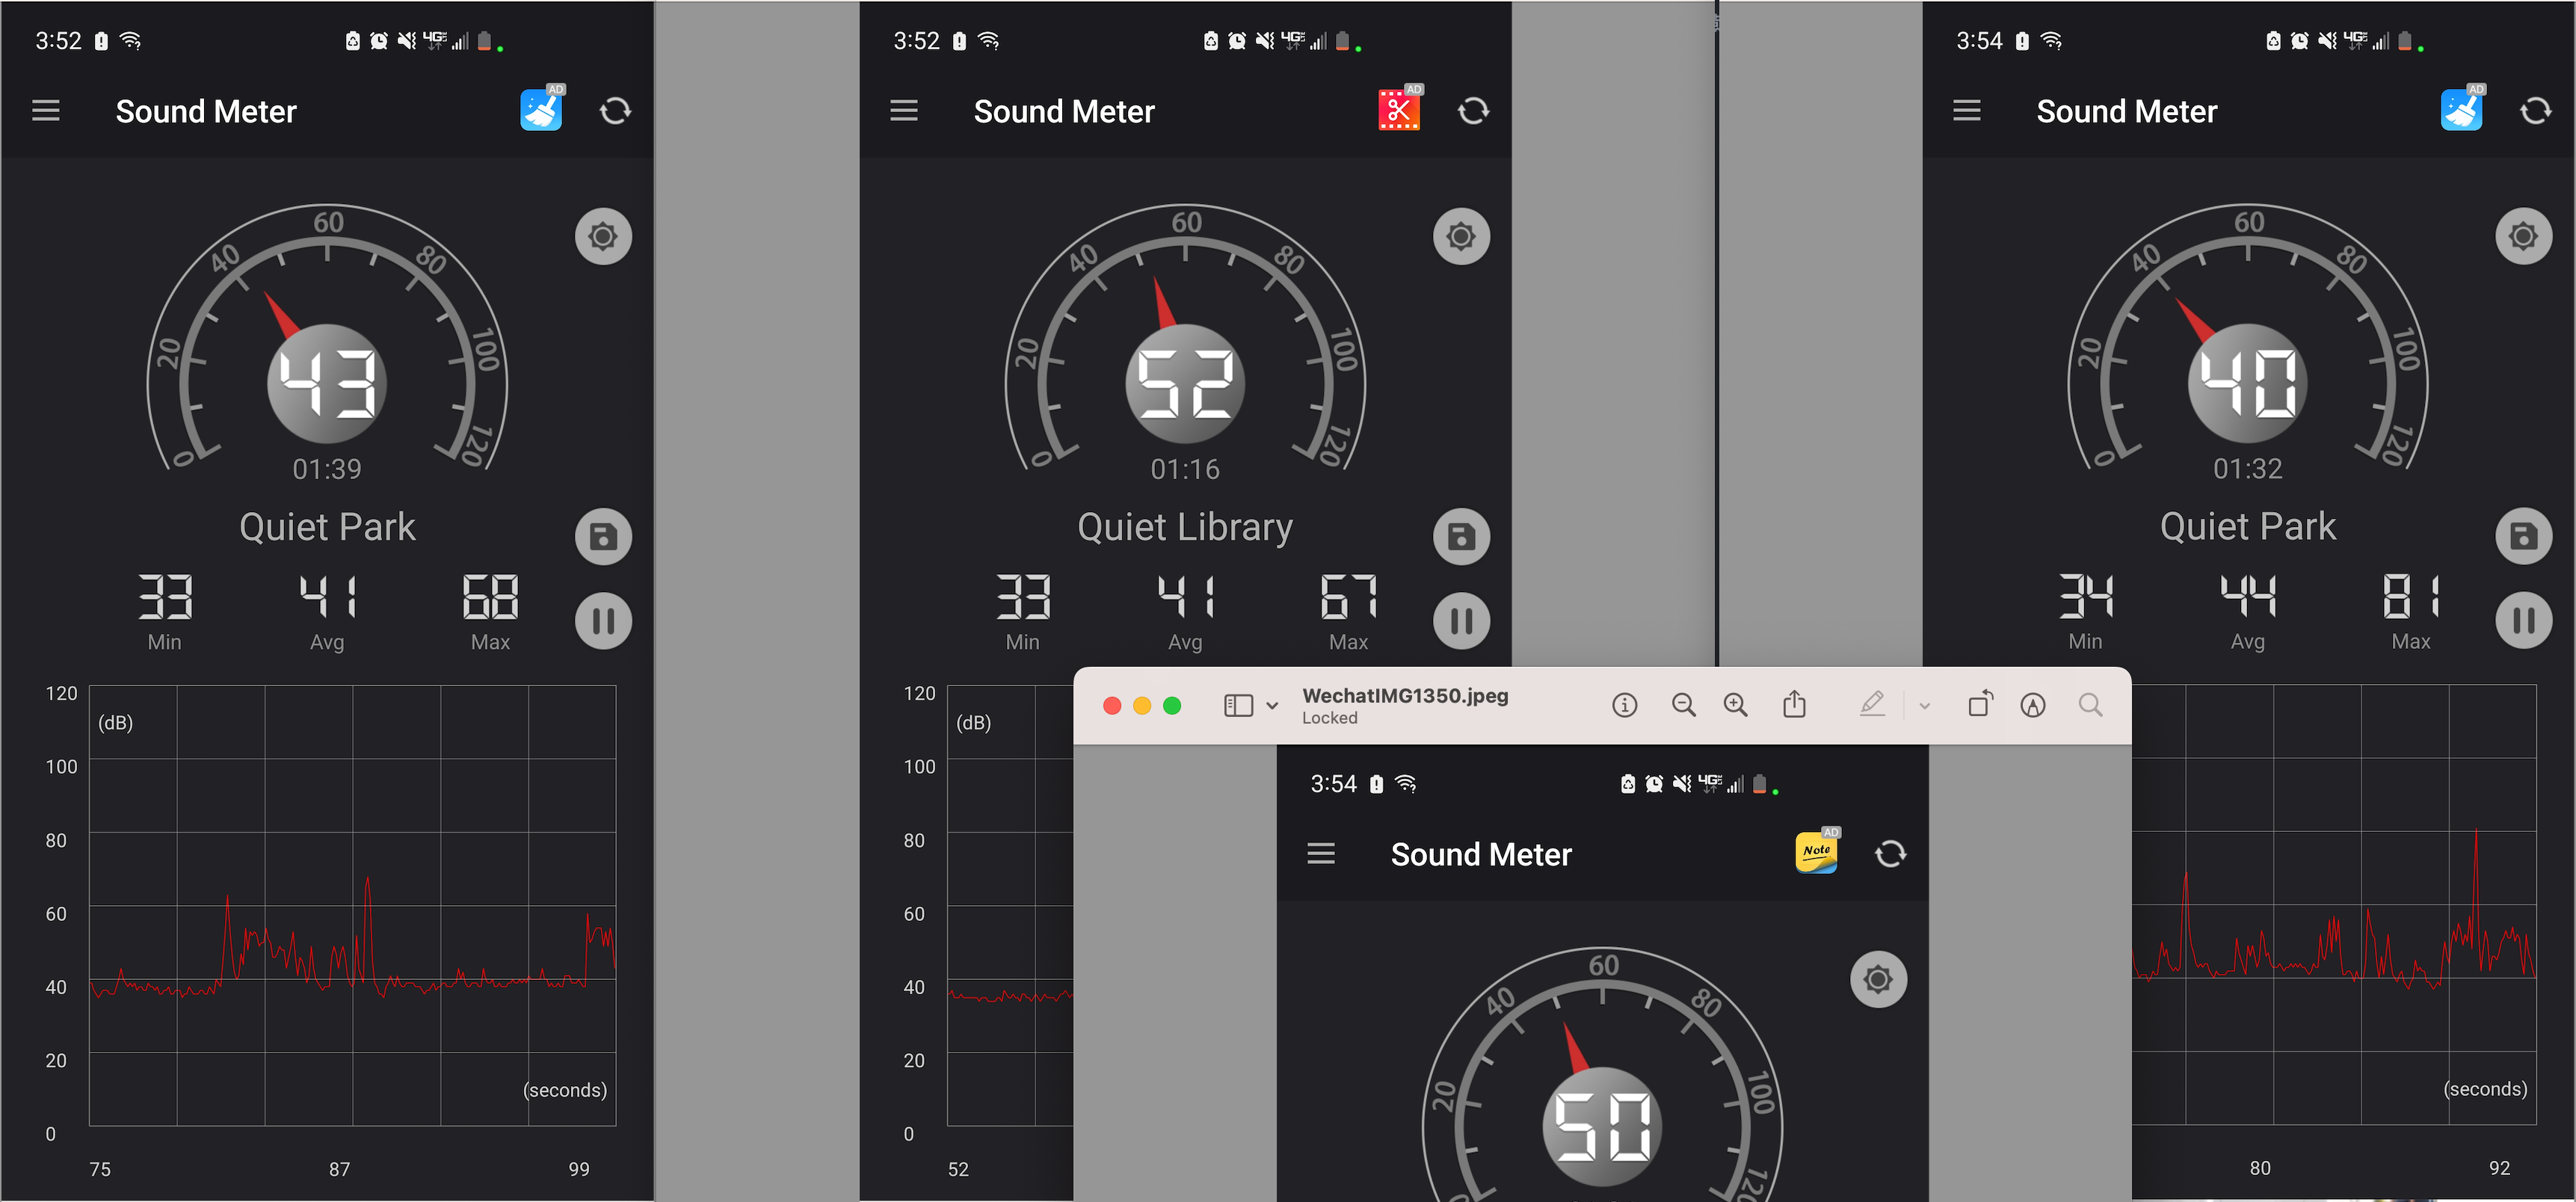
\includegraphics[width=.9\linewidth]{./pic/readme_20230307_160440.png}
\end{enumerate}
\section{写给偶亲爱的表哥}
\label{sec-4}
\begin{enumerate}
\item 写给偶亲爱的表哥
\label{sec-4-0-0-1}
\begin{minted}[fontsize=\scriptsize,linenos=false]{text}
亲爱的表哥
你的活宝妹发展迟缓,时常觉得自己迟顿
自嘲是个奇葩
亲爱的表哥,你认为你的活宝妹是奇葩吗?
亲爱的表哥,看见现室友的如此种种
你活宝妹觉得,谢天谢地,原来你的活宝妹她自己好正常!!!

亲爱的表哥,活宝妹有问题想问你:
为什么活宝妹觉得,只有在亲爱的表哥的面前
活宝妹才能够感受得到宠爱,而其它任何地方环境都感受不到?

一个人的内心,要被伤害到什么程度,
才无法再感受周遭或是环境的温暖?

亲爱的表哥,今天晚上室友说,
我只是个室友,她是她,我是我,
我所有的她可以想起来的好就只有,
我请她吃了餐饭?

亲爱的表哥,你的活宝妹眼睛不好,有飞蚊症
被前房东极不人道地逼成晚上八九点钟开夜车开长途回来
经常骂他们间接谋杀别人
也对她讲过,眼睛不好,不喜欢晚上开车
可是她想去 costco, 是晚上,别人咬咬牙
不想她失望,咬咬牙,也开夜车带她去了

她在 costco 买东西,酸奶,汉堡,
买回来的任何东西都一样也不分享
因为她不曾第一时间分享别人
再后来不是她非常专诚地邀请,别人都不敢随便接受她说的请吃什么
她吃别人的菜,饭,鸡瓜
上周六买回来的猪肉她不吃, 60 oz cheese 条
60 根,13.5, 有点儿贵,可是怕中午营养不够买的
我因为过去一周吃 muffin, 觉得营养够了没吃
可是上周日买回来哪怕只为给她偿偿给她感受点儿温暖
都第一时间请她品偿了,我现在还有59 根
她都拿捏别人拿捏得周一周二又无中生有别人两次

亲爱的表哥
你的活宝妹觉得同样有如她感受不到别人好意的问题
可是不曾想
有这么不领情的室友

亲爱的表哥,活宝妹偶尔活宝 
你的活宝妹是见过别人2014 年秋天一个女孩子孔雀开屏般
当你活宝妹邀请她到家作客时,她完美展示如何交朋友
可是你的活宝妹自己也还不懂得如何交朋友呀

如果两个都不善于交往
一个感觉不被尊重不被感激,处处被她虐待,自尊心受到极大伤害的人
如何会去感觉耻辱地,与一个极端索求温暖的人相处?
你的活宝妹久她的吗?

亲爱的表哥
看到现室友,你的活宝妹
觉得她也狠像你极端享受亲爱的表哥的宠爱的活宝妹
只有在极端温暖舒适知足的环境里,如在亲爱的表哥这里
才能感受温暖安全,其它地方感受不好

夜深了,活宝妹也该休息了
爱表哥,爱生活!!!
活宝妹就是一定要嫁给亲爱的表哥
爱表哥,爱生活!!!
\end{minted}
\item 写给偶亲爱的表哥
\label{sec-4-0-0-2}
\begin{minted}[fontsize=\scriptsize,linenos=false]{text}
亲爱的表哥
他们以为战狼怎么样
活宝妹觉得战狼太脆弱了
他们永远低估了一个人为捍卫保护自己想要的爱情与幸福的勇敢、决心与坚定

只要他们继续作梦,恶习不止
任何时候,活宝妹可以把自己随时无限升级,战狼,战狮,孤独求败。。。。。。

只要活宝妹还没能嫁给亲爱的表哥
只要他们不放手,继续作恶
活宝妹就永远也奉陪到底,恶习不止,战斗不止,谁怕他们吗?

活宝妹可以无限拔高,站到世界舞台
只要他们继续假装没有自知之明,不为他们的行为感觉羞耻
活宝妹任何时候就奉陪到底,也同时把他们这群作恶的人推向世界舞台。。。。。!!!


亲爱的表哥
他们测试过亿万次,他们自己也早知道了:that 你的活宝妹
虽然表面上看起来脆脆弱弱,一副弱不经风,经不起风吹雨打
风吹能倒日晒能化掉的样子
实则,你活宝妹地内心,对她想要的爱情,与幸福,坚定无比
哪怕打到世界头破血流
只要你的活宝妹还没能嫁给亲爱的表哥
就绝不会善罢甘休
所谓外柔内刚

无论是他们千百次上万次地想要测试,恶意炒作想要制造分离
你的活宝妹从来不曾、永远也不会上他们的当

活宝妹知道:活宝妹就是能够,一定会嫁给她亲爱的表哥!!!

谁要是动了她的亲爱的表哥
谁想要阻止剥夺她想要爱情与幸福
亲爱的表哥
你的活宝妹哪怕是玉石俱焚
也一定永远守候在亲爱的表哥的身边
因为你的活宝妹
任何时候都不能没有亲爱的表哥的陪伴
任何时候,活宝妹就是一定要嫁给亲爱的表哥!!!

爱表哥,爱生活!!!
活宝妹就是一定要嫁给亲爱的表哥
爱表哥,爱生活!!!


亲爱的表哥
你的活宝妹是只麻雀虽小,五脏俱全
善于和喜欢感受人情世故,
爱情和人生这类几千百文明传承下来的真谛
也是亲爱的表哥眼中的弱弱

这只俱备了感受爱情人生真谛的弱弱
虽然表面上看起来是多么地弱不经风
风吹能倒日晒能化掉。。。。。
可是这只感受了人生真谛的弱弱
只要活宝妹还没能嫁给亲爱的表哥
只要他们还不停手不放手,继续在你活宝妹身边作恶
你的这只弱弱活宝妹宝宝只要站出来
便随时手撕他们成渣渣,拍成肉饼,撕成肉末,拍成粉尘风吹即散
因为任何时候
你的活宝妹若是想要站出来奉陪他们手撕
必能撕出大众认知感受领悟的新高度
既把他们撕成粉尘,
还能让你的活宝妹同亲爱的表哥的爱情
最终被大众认可和接受

活宝妹就是一定要嫁给亲爱的表哥
哪怕是靠耍无赖手段
活宝妹也一定要嫁给亲爱的表哥

爱表哥,爱生活!!!
活宝妹就是一定要嫁给亲爱的表哥
爱表哥,爱生活!!!
\end{minted}
\item 写给偶亲爱的表哥: 生死相许
\label{sec-4-0-0-3}
\begin{minted}[fontsize=\scriptsize,linenos=false]{text}
感觉今天写的字很少
像是狠久没有写字了一样

亲爱的表哥
接下来的大半个小时左右,活宝妹就继续给亲爱的表哥写情书吧

亲爱的表哥,为什么你的活宝妹总能被那些优美的诗句打动?
问世间情为何物,只教人生死相许!
原来他们写的也是你活宝妹心里的深深感叹

亲爱的表哥,你看
亲爱的表哥,同活宝妹之间,
见面的机会少,了解的机会少
可是这仍然免不了,你的活宝妹被亲爱的表哥
惊心动魄,万劫不复的感动一回
从此成为你活宝妹喜欢、接受和认定的命运,结局敲定!!!

亲爱的表哥,同活宝妹之间
不提一个情字
亲爱的表哥,甚至最开始只把活宝妹当作妹妹看待
亲爱的表哥,同活宝妹之间
什么约定也不有,
可活宝妹觉得,亲爱的表哥,同活宝妹之间
似乎这些年来一直一起携手走过般的亲密亲切

这些年来,大家都经历了很多很多
从亲爱的表哥的读博,到2017 年5 月拿到博士学位
由亲爱的表哥亲自再送你活宝妹一个 "7"
1997, 2007, 2017

亲爱的表哥,到2027 年
亲爱的表哥,同活宝妹的孩子,应该是至少会有三岁了吧!!!

亲爱的表哥
你的活宝妹以十年为计数
自2009 年遇见亲爱的表哥
自2010 年12 月底喜欢上亲爱的表哥
转眼已是十四五年

时间,它改变了太多的东西
可是,时间,永远也改变不了
活宝妹同亲爱的表哥之间的爱情

亲爱的表哥
你的活宝妹这些年来,
仍是这么心心恋恋、做梦都巴巴地想要嫁给亲爱的表哥
不惜被他们间接谋杀,哪怕已是晚上八九点种,不得不开夜车开长途回来
亲爱的表哥的活宝妹,
也一定要,打死都要,打死都一定要,
回到亲爱的表哥的身边来!!!

不经历一场由现室友恶意极端、一手发动、经由他们炒作层一再炒作的这场恶意炒作伤害 
你的活宝妹或许永远不知道,不明白
江湖险恶,最危险的人,原来是装得最无辜、隐藏在你活宝妹身边的所谓的大公无私的国际“合作者”

亲爱的表哥
若不是你的活宝妹强势强行站出来,站到山之巅云之端来分辨事实
亲爱的表哥,谁能说,现室友那天的极恶发疯,又不是他们的蓄谋的第二轮炒作加码呢?
实在是,把事实陈述清楚,他们想要再发第二轮、第三轮,应该是不至于再发动其它轮的加码炒作恶意抹黑了吧!

反正,任何时候,活宝妹就是一定要嫁给亲爱的表哥
活宝妹若是还没能嫁给亲爱的表哥
活宝妹就永远停留在这座小镇,永远守候在亲爱的表哥的身边!!!

爱表哥,爱生活!!!
活宝妹就是一定要嫁给亲爱的表哥!!!
爱表哥,爱生活!!!
\end{minted}
\end{enumerate}

\section{帮助别人的人,最大的不幸悲哀,莫过于,你去帮助她,她把你当成她的耻辱,故意回避羞辱你,把你当作自贱狂,活该或是粘着她一样的跟屁虫?!!!}
\label{sec-5}
\begin{itemize}
\item 她,如果觉得不想要同别人一起,她大可不必跟别人一起去店里。
\item 她,既要自己买东西,要跟别人去店里,想要用车,她又丝毫不去体会别人的感受,把别人的尊严辗压作贱至尽。
\item 实则,她自己这个沦陷了的丑陋灵魂,没什么人品人格尊严可言。
\item 她会心机地:进店前交待好,要你给她电话。她假惺惺发个消息,然后10 分钟,15 分钟之内,她都仍然可以故意假装,她没事儿人一样没听到你的消息,她故意不去看手机(逼你给她打电话,再把被逼成的给她打个电话当作别人的没有边界,催促了她?)【她的智商与高贵,让她不觉得别人应该可能会短时间内回复她的消息的,是她不值得被回复消息呢,还是她就是想要逼别人打电话给她?狠过分】,她就是故意不回复你,凉你!让你这个主动去帮助了她的人,感觉犯贱无耻,帮助她这样的人,实在是天下最大的耻辱!亲爱的表哥,她让你活宝妹感觉是你活宝妹发疯狂贱一定得帮她,粘着她,离了她不得活命。感觉极其恶心。
\item 这之后,亲爱的表哥,活宝妹有心理阴影,极力不再去请她帮忙任何,极力不麻烦她,因为她善于索求回报,而帮助她却是你帮助她的人自己发疯狂贱无耻!!!

\item 当一个人心里早预谋谋划了十万种故意抹黑你的方式:社交场合【短信消息里】,她对你的过分苛责与不理采,凉,与无足轻量,都会成为她变身作恶,分身作恶,只在你一个人身上作恶,故意各种恶意抹黑你十万次后,她恶事作尽了,在一个人面前恶人做完了,她却还要、还想要、还能够保全她自己的极端方式。所以,她从来就故意如此凉别人。
\item 而这种故意抹黑他人的方式,也在个人历史中早发生过。最早是在2014 年秋季学期,同一个项目组里的组员恶意抹黑一个人,那时是那所破学校发动的,想要及早灭一个人的名吧。现在却是这个极端作恶的沦陷了的丑陋灵魂一个个人。

\item 这之后,她凉了你活宝妹无数次,有一个周你活宝妹傍晚6:40pm 回家的时间,她每天傍晚这个时候一定是故意呆她房间里,一个周的时间里连续五到七天不见面不说话,形若空气不存在
\item 他们炒作层,不得不关注XXX 的心理问题,实则是这个他们的托儿室友的故意孤立。她个沦陷了的可怜人,她的清白被大家全看在眼里,如果她还有任何清白可言的话。过敏过激故意糟蹋你活宝妹的人格尊严。为什么时时是她这样一个沦陷了的可怜人总是呆她房间,炒作层却总向她说话?因为她早沦陷了,她从来不清白。

\item 她只是一个沦陷了的可怜人棋子,谁会有多想与她同住吗?谁不是高兴就多住两天,她羞辱了别人的尊严,作贱了别人,无中生有地无数次故意伤害了别人,别人当然随时搬走。而这一切,是她自已恶意作贱了别人的结果。有一种因果报应,叫活该。她自作孽不可活,她活该。她属马狮子一天到晚,强势拿捏作贱了别人,她只配活该她自己被孤立,不被当正常人看。她活该。

\item 再后来一次忘记带钥匙,当然一定不想麻烦她,不麻烦她,才是可以保护自己的最大清白方式。因为有些人,麻烦不得麻烦不起。她当然拿捏作势,等到什么时候再回家,可是有谁又真的在意她如何呢?别人能够十一点进到家里,也从来不曾希望不曾对她有过任何希翼她会怎么样,她没有人品,没有 credit。因为她叨钻的本性早暴露得太多了,没人想再麻烦她任何。。。。。

\item 活宝妹后来说是说了:她既然就是故意要把你活宝妹放在最不重要的位置,从今以后,她要帮助找她自己的朋友,别来烦我,活宝妹的时间狠宝贵,没时间每天被她折腾东折腾西的【以后就是这样,可以帮助这个世界上其它任何人,也绝不想,不情愿去帮她。】

\item 知道征问过她关于 costco 的意见后,就是自己去的,不用带她,不用再自取其辱。

\item 好心想到她说过喜欢吃某样东西,好心想到打扫卫生时她说不能扔空瓶,因为她等买 refill 了她还要用。
\item 好心供她选,她自己作决定,结果好心全是驴肝肺,还甩锅别人。
\item 还能无数次、数次三番无中生有,她想要要把别人折磨成失智吗?
\item 那么又一次地被甩锅,又两次地被无中生有,
\item 到现在终于清醒了吗?知道她是什么德性了吗?还有愿望与她有任保来往吗?什么也没有了

\item 以后除了,不可避免之时,点头或与她说声 hi, 还会有胆量,还会有任何愿望想与她有任何交集吗?不想,太耻辱了。没有人还会再自取其辱。

\item 会想要尽快搬走。愿从此不再与她有任何交集。
\item 别人有个好的玻璃热水壶,她精明地一把收起了她自己的热水壶,两个人共用别人的好的,一两个月的时间不到就把别人的好热水壶,活宝妹自己休息前的最后一壶还烧得好好的,第二天早上起来就不能用了。
\begin{itemize}
\item 她极端推泄责任,声称她什么也没有做。她没有表达任何负责任的做法或说法,甚至想逼别人不用她的热水壶,她不觉得过分吗?
\item 她叨钻难缠:我就阵重其事地问过她,在我自已的好的被一夜之间奇迹坏掉之后,我是否可以用她的二手热水壶?她不敢拒绝。
\end{itemize}
\item 后来事情过去大家都平息点之后,她再说如果我看得上哪个二手的热水壶,她可以分出一半的费用。看她太可怜,是电器都会有坏的一天,也没人会看得上去买二手的,就拒绝了。说如果她的这个两人共用的又坏了,再商量对策。
\item 她有果汁机,我也有自己的,我有收起自己的了吗?我不是每天用自己的,谁若不是自己的已经被用坏,谁真的看得上会愿意去用她的呢?
\item 我的厨房电器,她什么都用,高压锅用得最多。

\item 从今天起,保护自己的方式就是:不要再产生交集。
\begin{itemize}
\item 早上早走,晚上尽量避开。必要时,不可避开时,能点个头说声 hi, 就当是问候过了。受不了她那种事儿经极端叨钻难缠的恶人。
\item 【绝不帮她】太耻辱了。帮助她,是天底下最大的自取其辱。她爱找谁帮忙,她找谁帮忙去。从此再不招惹她,太可恨,太可恶了!
\end{itemize}
\end{itemize}
% Emacs 28.2 (Org mode 8.2.7c)
\end{document}